\documentclass[1p]{elsarticle_modified}
%\bibliographystyle{elsarticle-num}

%\usepackage[colorlinks]{hyperref}
%\usepackage{abbrmath_seonhwa} %\Abb, \Ascr, \Acal ,\Abf, \Afrak
\usepackage{amsfonts}
\usepackage{amssymb}
\usepackage{amsmath}
\usepackage{amsthm}
\usepackage{scalefnt}
\usepackage{amsbsy}
\usepackage{kotex}
\usepackage{caption}
\usepackage{subfig}
\usepackage{color}
\usepackage{graphicx}
\usepackage{xcolor} %% white, black, red, green, blue, cyan, magenta, yellow
\usepackage{float}
\usepackage{setspace}
\usepackage{hyperref}

\usepackage{tikz}
\usetikzlibrary{arrows}

\usepackage{multirow}
\usepackage{array} % fixed length table
\usepackage{hhline}

%%%%%%%%%%%%%%%%%%%%%
\makeatletter
\renewcommand*\env@matrix[1][\arraystretch]{%
	\edef\arraystretch{#1}%
	\hskip -\arraycolsep
	\let\@ifnextchar\new@ifnextchar
	\array{*\c@MaxMatrixCols c}}
\makeatother %https://tex.stackexchange.com/questions/14071/how-can-i-increase-the-line-spacing-in-a-matrix
%%%%%%%%%%%%%%%

\usepackage[normalem]{ulem}

\newcommand{\msout}[1]{\ifmmode\text{\sout{\ensuremath{#1}}}\else\sout{#1}\fi}
%SOURCE: \msout is \stkout macro in https://tex.stackexchange.com/questions/20609/strikeout-in-math-mode

\newcommand{\cancel}[1]{
	\ifmmode
	{\color{red}\msout{#1}}
	\else
	{\color{red}\sout{#1}}
	\fi
}

\newcommand{\add}[1]{
	{\color{blue}\uwave{#1}}
}

\newcommand{\replace}[2]{
	\ifmmode
	{\color{red}\msout{#1}}{\color{blue}\uwave{#2}}
	\else
	{\color{red}\sout{#1}}{\color{blue}\uwave{#2}}
	\fi
}

\newcommand{\Sol}{\mathcal{S}} %segment
\newcommand{\D}{D} %diagram
\newcommand{\A}{\mathcal{A}} %arc


%%%%%%%%%%%%%%%%%%%%%%%%%%%%%5 test

\def\sl{\operatorname{\textup{SL}}(2,\Cbb)}
\def\psl{\operatorname{\textup{PSL}}(2,\Cbb)}
\def\quan{\mkern 1mu \triangleright \mkern 1mu}

\theoremstyle{definition}
\newtheorem{thm}{Theorem}[section]
\newtheorem{prop}[thm]{Proposition}
\newtheorem{lem}[thm]{Lemma}
\newtheorem{ques}[thm]{Question}
\newtheorem{cor}[thm]{Corollary}
\newtheorem{defn}[thm]{Definition}
\newtheorem{exam}[thm]{Example}
\newtheorem{rmk}[thm]{Remark}
\newtheorem{alg}[thm]{Algorithm}

\newcommand{\I}{\sqrt{-1}}
\begin{document}

%\begin{frontmatter}
%
%\title{Boundary parabolic representations of knots up to 8 crossings}
%
%%% Group authors per affiliation:
%\author{Yunhi Cho} 
%\address{Department of Mathematics, University of Seoul, Seoul, Korea}
%\ead{yhcho@uos.ac.kr}
%
%
%\author{Seonhwa Kim} %\fnref{s_kim}}
%\address{Center for Geometry and Physics, Institute for Basic Science, Pohang, 37673, Korea}
%\ead{ryeona17@ibs.re.kr}
%
%\author{Hyuk Kim}
%\address{Department of Mathematical Sciences, Seoul National University, Seoul 08826, Korea}
%\ead{hyukkim@snu.ac.kr}
%
%\author{Seokbeom Yoon}
%\address{Department of Mathematical Sciences, Seoul National University, Seoul, 08826,  Korea}
%\ead{sbyoon15@snu.ac.kr}
%
%\begin{abstract}
%We find all boundary parabolic representation of knots up to 8 crossings.
%
%\end{abstract}
%\begin{keyword}
%    \MSC[2010] 57M25 
%\end{keyword}
%
%\end{frontmatter}

%\linenumbers
%\tableofcontents
%
\newcommand\colored[1]{\textcolor{white}{\rule[-0.35ex]{0.8em}{1.4ex}}\kern-0.8em\color{red} #1}%
%\newcommand\colored[1]{\textcolor{white}{ #1}\kern-2.17ex	\textcolor{white}{ #1}\kern-1.81ex	\textcolor{white}{ #1}\kern-2.15ex\color{red}#1	}

{\Large $\underline{11a_{18}~(K11a_{18})}$}

\setlength{\tabcolsep}{10pt}
\renewcommand{\arraystretch}{1.6}
\vspace{1cm}\begin{tabular}{m{100pt}>{\centering\arraybackslash}m{274pt}}
\multirow{5}{120pt}{
	\centering
	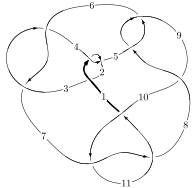
\includegraphics[width=112pt]{../../../GIT/diagram.site/Diagrams/png/267_11a_18.png}\\
\ \ \ A knot diagram\footnotemark}&
\allowdisplaybreaks
\textbf{Linearized knot diagam} \\
\cline{2-2}
 &
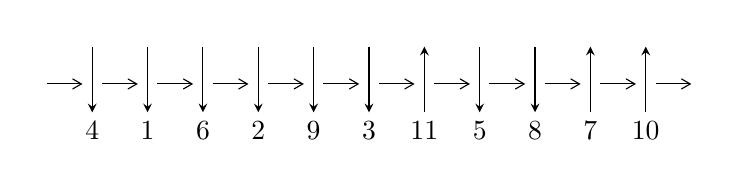
\begin{tikzpicture}[x=20pt, y=17pt]
	% nodes
	\node (C0) at (0, 0) {};
	\node (C1) at (1, 0) {};
	\node (C1U) at (1, +1) {};
	\node (C1D) at (1, -1) {4};

	\node (C2) at (2, 0) {};
	\node (C2U) at (2, +1) {};
	\node (C2D) at (2, -1) {1};

	\node (C3) at (3, 0) {};
	\node (C3U) at (3, +1) {};
	\node (C3D) at (3, -1) {6};

	\node (C4) at (4, 0) {};
	\node (C4U) at (4, +1) {};
	\node (C4D) at (4, -1) {2};

	\node (C5) at (5, 0) {};
	\node (C5U) at (5, +1) {};
	\node (C5D) at (5, -1) {9};

	\node (C6) at (6, 0) {};
	\node (C6U) at (6, +1) {};
	\node (C6D) at (6, -1) {3};

	\node (C7) at (7, 0) {};
	\node (C7U) at (7, +1) {};
	\node (C7D) at (7, -1) {11};

	\node (C8) at (8, 0) {};
	\node (C8U) at (8, +1) {};
	\node (C8D) at (8, -1) {5};

	\node (C9) at (9, 0) {};
	\node (C9U) at (9, +1) {};
	\node (C9D) at (9, -1) {8};

	\node (C10) at (10, 0) {};
	\node (C10U) at (10, +1) {};
	\node (C10D) at (10, -1) {7};

	\node (C11) at (11, 0) {};
	\node (C11U) at (11, +1) {};
	\node (C11D) at (11, -1) {10};
	\node (C12) at (12, 0) {};

	% arrows
	\draw[->,>={angle 60}]
	(C0) edge (C1) (C1) edge (C2) (C2) edge (C3) (C3) edge (C4) (C4) edge (C5) (C5) edge (C6) (C6) edge (C7) (C7) edge (C8) (C8) edge (C9) (C9) edge (C10) (C10) edge (C11) (C11) edge (C12) ;	\draw[->,>=stealth]
	(C1U) edge (C1D) (C2U) edge (C2D) (C3U) edge (C3D) (C4U) edge (C4D) (C5U) edge (C5D) (C6U) edge (C6D) (C7D) edge (C7U) (C8U) edge (C8D) (C9U) edge (C9D) (C10D) edge (C10U) (C11D) edge (C11U) ;
	\end{tikzpicture} \\
\hhline{~~} \\& 
\textbf{Solving Sequence} \\ \cline{2-2} 
 &
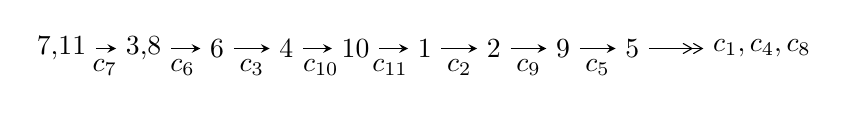
\begin{tikzpicture}[x=25pt, y=7pt]
	% node
	\node (A0) at (-1/8, 0) {7,11};
	\node (A1) at (17/16, 0) {3,8};
	\node (A2) at (17/8, 0) {6};
	\node (A3) at (25/8, 0) {4};
	\node (A4) at (33/8, 0) {10};
	\node (A5) at (41/8, 0) {1};
	\node (A6) at (49/8, 0) {2};
	\node (A7) at (57/8, 0) {9};
	\node (A8) at (65/8, 0) {5};
	\node (C1) at (1/2, -1) {$c_{7}$};
	\node (C2) at (13/8, -1) {$c_{6}$};
	\node (C3) at (21/8, -1) {$c_{3}$};
	\node (C4) at (29/8, -1) {$c_{10}$};
	\node (C5) at (37/8, -1) {$c_{11}$};
	\node (C6) at (45/8, -1) {$c_{2}$};
	\node (C7) at (53/8, -1) {$c_{9}$};
	\node (C8) at (61/8, -1) {$c_{5}$};
	\node (A9) at (10, 0) {$c_{1},c_{4},c_{8}$};

	% edge
	\draw[->,>=stealth]	
	(A0) edge (A1) (A1) edge (A2) (A2) edge (A3) (A3) edge (A4) (A4) edge (A5) (A5) edge (A6) (A6) edge (A7) (A7) edge (A8) ;
	\draw[->>,>={angle 60}]	
	(A8) edge (A9);
\end{tikzpicture} \\ 

\end{tabular} \\

\footnotetext{
The image of knot diagram is generated by the software ``\textbf{Draw programme}" developed by Andrew Bartholomew(\url{http://www.layer8.co.uk/maths/draw/index.htm\#Running-draw}), where we modified some parts for our purpose(\url{https://github.com/CATsTAILs/LinksPainter}).
}\phantom \\ \newline 
\centering \textbf{Ideals for irreducible components\footnotemark of $X_{\text{par}}$} 
 
\begin{align*}
I^u_{1}&=\langle 
-2.02368\times10^{22} u^{71}+1.11016\times10^{23} u^{70}+\cdots+1.88857\times10^{22} b-6.09914\times10^{22},\\
\phantom{I^u_{1}}&\phantom{= \langle  }4.07828\times10^{22} u^{71}-1.25681\times10^{23} u^{70}+\cdots+3.77714\times10^{22} a+1.39984\times10^{23},\;u^{72}-5 u^{71}+\cdots+12 u-1\rangle \\
I^u_{2}&=\langle 
b,\;u^3- u^2+a+1,\;u^6- u^5- u^4+2 u^3- u+1\rangle \\
I^u_{3}&=\langle 
a^2+5 b+3 a+5,\;a^3+a^2+4 a+5,\;u+1\rangle \\
\\
\end{align*}
\raggedright * 3 irreducible components of $\dim_{\mathbb{C}}=0$, with total 81 representations.\\
\footnotetext{All coefficients of polynomials are rational numbers. But the coefficients are sometimes approximated in decimal forms when there is not enough margin.}
\newpage
\renewcommand{\arraystretch}{1}
\centering \section*{I. $I^u_{1}= \langle -2.02\times10^{22} u^{71}+1.11\times10^{23} u^{70}+\cdots+1.89\times10^{22} b-6.10\times10^{22},\;4.08\times10^{22} u^{71}-1.26\times10^{23} u^{70}+\cdots+3.78\times10^{22} a+1.40\times10^{23},\;u^{72}-5 u^{71}+\cdots+12 u-1 \rangle$}
\flushleft \textbf{(i) Arc colorings}\\
\begin{tabular}{m{7pt} m{180pt} m{7pt} m{180pt} }
\flushright $a_{7}=$&$\begin{pmatrix}1\\0\end{pmatrix}$ \\
\flushright $a_{11}=$&$\begin{pmatrix}0\\u\end{pmatrix}$ \\
\flushright $a_{3}=$&$\begin{pmatrix}-1.07973 u^{71}+3.32742 u^{70}+\cdots+8.79814 u-3.70610\\1.07154 u^{71}-5.87833 u^{70}+\cdots-27.8922 u+3.22950\end{pmatrix}$ \\
\flushright $a_{8}=$&$\begin{pmatrix}1\\- u^2\end{pmatrix}$ \\
\flushright $a_{6}=$&$\begin{pmatrix}7.15660 u^{71}-30.9077 u^{70}+\cdots-110.914 u+13.1587\\-3.05252 u^{71}+13.6578 u^{70}+\cdots+48.6687 u-4.93370\end{pmatrix}$ \\
\flushright $a_{4}=$&$\begin{pmatrix}-8.96090 u^{71}+37.1749 u^{70}+\cdots+124.175 u-16.1656\\6.60610 u^{71}-29.5950 u^{70}+\cdots-105.720 u+10.6845\end{pmatrix}$ \\
\flushright $a_{10}=$&$\begin{pmatrix}- u\\u\end{pmatrix}$ \\
\flushright $a_{1}=$&$\begin{pmatrix}u^3\\- u^3+u\end{pmatrix}$ \\
\flushright $a_{2}=$&$\begin{pmatrix}-1.44106 u^{71}+6.20595 u^{70}+\cdots+24.5011 u-5.21118\\-0.925198 u^{71}+1.52843 u^{70}+\cdots-9.87376 u+1.65560\end{pmatrix}$ \\
\flushright $a_{9}=$&$\begin{pmatrix}- u^3\\u^5- u^3+u\end{pmatrix}$ \\
\flushright $a_{5}=$&$\begin{pmatrix}6.74498 u^{71}-26.4676 u^{70}+\cdots-87.3523 u+10.9648\\-6.68660 u^{71}+26.6048 u^{70}+\cdots+77.8117 u-7.58573\end{pmatrix}$\\ \flushright $a_{5}=$&$\begin{pmatrix}6.74498 u^{71}-26.4676 u^{70}+\cdots-87.3523 u+10.9648\\-6.68660 u^{71}+26.6048 u^{70}+\cdots+77.8117 u-7.58573\end{pmatrix}$\\&\end{tabular}
\flushleft \textbf{(ii) Obstruction class $= -1$}\\~\\
\flushleft \textbf{(iii) Cusp Shapes $= -\frac{76710752927736823653759}{9442837768770389262581} u^{71}+\frac{509177888669513108789191}{18885675537540778525162} u^{70}+\cdots+\frac{316804939896701446179690}{9442837768770389262581} u-\frac{245852902489482612469787}{18885675537540778525162}$}\\~\\
\newpage\renewcommand{\arraystretch}{1}
\flushleft \textbf{(iv) u-Polynomials at the component}\newline \\
\begin{tabular}{m{50pt}|m{274pt}}
Crossings & \hspace{64pt}u-Polynomials at each crossing \\
\hline $$\begin{aligned}c_{1},c_{4}\end{aligned}$$&$\begin{aligned}
&u^{72}-8 u^{71}+\cdots-12 u+1
\end{aligned}$\\
\hline $$\begin{aligned}c_{2}\end{aligned}$$&$\begin{aligned}
&u^{72}+32 u^{71}+\cdots-8 u+1
\end{aligned}$\\
\hline $$\begin{aligned}c_{3},c_{6}\end{aligned}$$&$\begin{aligned}
&u^{72}-2 u^{71}+\cdots+128 u-64
\end{aligned}$\\
\hline $$\begin{aligned}c_{5},c_{8}\end{aligned}$$&$\begin{aligned}
&u^{72}+2 u^{71}+\cdots+20 u+8
\end{aligned}$\\
\hline $$\begin{aligned}c_{7},c_{10}\end{aligned}$$&$\begin{aligned}
&u^{72}+5 u^{71}+\cdots-12 u-1
\end{aligned}$\\
\hline $$\begin{aligned}c_{9}\end{aligned}$$&$\begin{aligned}
&u^{72}+24 u^{71}+\cdots+1872 u+64
\end{aligned}$\\
\hline $$\begin{aligned}c_{11}\end{aligned}$$&$\begin{aligned}
&u^{72}-39 u^{71}+\cdots-52 u+1
\end{aligned}$\\
\hline
\end{tabular}\\~\\
\newpage\renewcommand{\arraystretch}{1}
\flushleft \textbf{(v) Riley Polynomials at the component}\newline \\
\begin{tabular}{m{50pt}|m{274pt}}
Crossings & \hspace{64pt}Riley Polynomials at each crossing \\
\hline $$\begin{aligned}c_{1},c_{4}\end{aligned}$$&$\begin{aligned}
&y^{72}-32 y^{71}+\cdots+8 y+1
\end{aligned}$\\
\hline $$\begin{aligned}c_{2}\end{aligned}$$&$\begin{aligned}
&y^{72}+24 y^{71}+\cdots+2568 y+1
\end{aligned}$\\
\hline $$\begin{aligned}c_{3},c_{6}\end{aligned}$$&$\begin{aligned}
&y^{72}+42 y^{71}+\cdots+73728 y+4096
\end{aligned}$\\
\hline $$\begin{aligned}c_{5},c_{8}\end{aligned}$$&$\begin{aligned}
&y^{72}-24 y^{71}+\cdots-1872 y+64
\end{aligned}$\\
\hline $$\begin{aligned}c_{7},c_{10}\end{aligned}$$&$\begin{aligned}
&y^{72}-39 y^{71}+\cdots-52 y+1
\end{aligned}$\\
\hline $$\begin{aligned}c_{9}\end{aligned}$$&$\begin{aligned}
&y^{72}+44 y^{71}+\cdots-601344 y+4096
\end{aligned}$\\
\hline $$\begin{aligned}c_{11}\end{aligned}$$&$\begin{aligned}
&y^{72}-7 y^{71}+\cdots-2176 y+1
\end{aligned}$\\
\hline
\end{tabular}\\~\\
\newpage\flushleft \textbf{(vi) Complex Volumes and Cusp Shapes}
$$\begin{array}{c|c|c}  
\text{Solutions to }I^u_{1}& \I (\text{vol} + \sqrt{-1}CS) & \text{Cusp shape}\\
 \hline 
\begin{aligned}
u &= -0.876128 + 0.485866 I \\
a &= -1.020580 - 0.525723 I \\
b &= \phantom{-}0.151401 - 0.941501 I\end{aligned}
 & \phantom{-}1.78878 + 0.06007 I & \phantom{-0.000000 } 0 \\ \hline\begin{aligned}
u &= -0.876128 - 0.485866 I \\
a &= -1.020580 + 0.525723 I \\
b &= \phantom{-}0.151401 + 0.941501 I\end{aligned}
 & \phantom{-}1.78878 - 0.06007 I & \phantom{-0.000000 } 0 \\ \hline\begin{aligned}
u &= \phantom{-}0.642602 + 0.759427 I \\
a &= -0.004406 - 0.268942 I \\
b &= -0.468956 - 0.932444 I\end{aligned}
 & -3.84415 - 3.26268 I & \phantom{-0.000000 } 0 \\ \hline\begin{aligned}
u &= \phantom{-}0.642602 - 0.759427 I \\
a &= -0.004406 + 0.268942 I \\
b &= -0.468956 + 0.932444 I\end{aligned}
 & -3.84415 + 3.26268 I & \phantom{-0.000000 } 0 \\ \hline\begin{aligned}
u &= \phantom{-}0.809332 + 0.576281 I \\
a &= -0.308570 + 0.160474 I \\
b &= -0.794967 - 0.622629 I\end{aligned}
 & -4.30882 + 3.51764 I & \phantom{-0.000000 } 0 \\ \hline\begin{aligned}
u &= \phantom{-}0.809332 - 0.576281 I \\
a &= -0.308570 - 0.160474 I \\
b &= -0.794967 + 0.622629 I\end{aligned}
 & -4.30882 - 3.51764 I & \phantom{-0.000000 } 0 \\ \hline\begin{aligned}
u &= -0.951216 + 0.225981 I \\
a &= -0.764228 + 0.449018 I \\
b &= -0.173093 - 0.363920 I\end{aligned}
 & \phantom{-}1.73034 - 0.74165 I & \phantom{-0.000000 } 0 \\ \hline\begin{aligned}
u &= -0.951216 - 0.225981 I \\
a &= -0.764228 - 0.449018 I \\
b &= -0.173093 + 0.363920 I\end{aligned}
 & \phantom{-}1.73034 + 0.74165 I & \phantom{-0.000000 } 0 \\ \hline\begin{aligned}
u &= -1.05211\phantom{ +0.000000I} \\
a &= -2.54516\phantom{ +0.000000I} \\
b &= -0.432247\phantom{ +0.000000I}\end{aligned}
 & \phantom{-}0.330921\phantom{ +0.000000I} & -46.0800\phantom{ +0.000000I} \\ \hline\begin{aligned}
u &= \phantom{-}0.914907 + 0.540239 I \\
a &= \phantom{-}0.652730 + 1.039110 I \\
b &= \phantom{-}0.571615 - 0.771611 I\end{aligned}
 & -0.63477 + 4.40212 I & \phantom{-0.000000 } 0\\
 \hline 
 \end{array}$$\newpage$$\begin{array}{c|c|c}  
\text{Solutions to }I^u_{1}& \I (\text{vol} + \sqrt{-1}CS) & \text{Cusp shape}\\
 \hline 
\begin{aligned}
u &= \phantom{-}0.914907 - 0.540239 I \\
a &= \phantom{-}0.652730 - 1.039110 I \\
b &= \phantom{-}0.571615 + 0.771611 I\end{aligned}
 & -0.63477 - 4.40212 I & \phantom{-0.000000 } 0 \\ \hline\begin{aligned}
u &= \phantom{-}0.729237 + 0.575747 I \\
a &= -1.30537 - 1.48267 I \\
b &= -0.617113 + 0.726794 I\end{aligned}
 & -4.53906 + 1.05261 I & -10.58932 - 3.82745 I \\ \hline\begin{aligned}
u &= \phantom{-}0.729237 - 0.575747 I \\
a &= -1.30537 + 1.48267 I \\
b &= -0.617113 - 0.726794 I\end{aligned}
 & -4.53906 - 1.05261 I & -10.58932 + 3.82745 I \\ \hline\begin{aligned}
u &= \phantom{-}0.199115 + 0.897753 I \\
a &= -0.610450 + 0.607154 I \\
b &= -0.64956 - 1.25765 I\end{aligned}
 & \phantom{-}1.48181 - 10.73100 I & -6.00773 + 7.14911 I \\ \hline\begin{aligned}
u &= \phantom{-}0.199115 - 0.897753 I \\
a &= -0.610450 - 0.607154 I \\
b &= -0.64956 + 1.25765 I\end{aligned}
 & \phantom{-}1.48181 + 10.73100 I & -6.00773 - 7.14911 I \\ \hline\begin{aligned}
u &= \phantom{-}0.453294 + 0.792285 I \\
a &= -0.230638 + 0.142154 I \\
b &= -0.207389 + 0.782148 I\end{aligned}
 & -2.85223 + 0.05705 I & -5.94816 - 3.77217 I \\ \hline\begin{aligned}
u &= \phantom{-}0.453294 - 0.792285 I \\
a &= -0.230638 - 0.142154 I \\
b &= -0.207389 - 0.782148 I\end{aligned}
 & -2.85223 - 0.05705 I & -5.94816 + 3.77217 I \\ \hline\begin{aligned}
u &= \phantom{-}0.151325 + 0.858429 I \\
a &= \phantom{-}0.338744 - 0.734808 I \\
b &= \phantom{-}0.435835 + 1.280920 I\end{aligned}
 & \phantom{-}3.59461 - 4.95936 I & -3.13446 + 3.17768 I \\ \hline\begin{aligned}
u &= \phantom{-}0.151325 - 0.858429 I \\
a &= \phantom{-}0.338744 + 0.734808 I \\
b &= \phantom{-}0.435835 - 1.280920 I\end{aligned}
 & \phantom{-}3.59461 + 4.95936 I & -3.13446 - 3.17768 I \\ \hline\begin{aligned}
u &= -0.686903 + 0.514666 I \\
a &= \phantom{-}1.257030 + 0.541255 I \\
b &= \phantom{-}0.337786 + 1.041550 I\end{aligned}
 & \phantom{-}1.23521 - 4.19775 I & -3.49766 + 6.68711 I\\
 \hline 
 \end{array}$$\newpage$$\begin{array}{c|c|c}  
\text{Solutions to }I^u_{1}& \I (\text{vol} + \sqrt{-1}CS) & \text{Cusp shape}\\
 \hline 
\begin{aligned}
u &= -0.686903 - 0.514666 I \\
a &= \phantom{-}1.257030 - 0.541255 I \\
b &= \phantom{-}0.337786 - 1.041550 I\end{aligned}
 & \phantom{-}1.23521 + 4.19775 I & -3.49766 - 6.68711 I \\ \hline\begin{aligned}
u &= \phantom{-}0.921196 + 0.680248 I \\
a &= -1.079360 - 0.688931 I \\
b &= -0.563006 + 1.013540 I\end{aligned}
 & -3.02672 + 8.64627 I & \phantom{-0.000000 } 0 \\ \hline\begin{aligned}
u &= \phantom{-}0.921196 - 0.680248 I \\
a &= -1.079360 + 0.688931 I \\
b &= -0.563006 - 1.013540 I\end{aligned}
 & -3.02672 - 8.64627 I & \phantom{-0.000000 } 0 \\ \hline\begin{aligned}
u &= \phantom{-}0.190668 + 0.789710 I \\
a &= -0.539342 - 0.183142 I \\
b &= -1.048020 + 0.360828 I\end{aligned}
 & -1.37174 - 4.55999 I & -7.56588 + 4.82929 I \\ \hline\begin{aligned}
u &= \phantom{-}0.190668 - 0.789710 I \\
a &= -0.539342 + 0.183142 I \\
b &= -1.048020 - 0.360828 I\end{aligned}
 & -1.37174 + 4.55999 I & -7.56588 - 4.82929 I \\ \hline\begin{aligned}
u &= \phantom{-}0.803990 + 0.062025 I \\
a &= \phantom{-}0.01110 + 2.46502 I \\
b &= \phantom{-}0.188498 - 1.395620 I\end{aligned}
 & \phantom{-}4.16423 + 3.00649 I & -10.90678 - 5.59644 I \\ \hline\begin{aligned}
u &= \phantom{-}0.803990 - 0.062025 I \\
a &= \phantom{-}0.01110 - 2.46502 I \\
b &= \phantom{-}0.188498 + 1.395620 I\end{aligned}
 & \phantom{-}4.16423 - 3.00649 I & -10.90678 + 5.59644 I \\ \hline\begin{aligned}
u &= -1.135490 + 0.370936 I \\
a &= \phantom{-}1.07671 - 2.69128 I \\
b &= \phantom{-}0.062046 + 0.875399 I\end{aligned}
 & \phantom{-}1.26979 - 1.25057 I & \phantom{-0.000000 } 0 \\ \hline\begin{aligned}
u &= -1.135490 - 0.370936 I \\
a &= \phantom{-}1.07671 + 2.69128 I \\
b &= \phantom{-}0.062046 - 0.875399 I\end{aligned}
 & \phantom{-}1.26979 + 1.25057 I & \phantom{-0.000000 } 0 \\ \hline\begin{aligned}
u &= \phantom{-}1.148040 + 0.380216 I \\
a &= -0.70878 - 1.85544 I \\
b &= \phantom{-}0.49043 + 1.40149 I\end{aligned}
 & \phantom{-}6.72982 - 1.38866 I & \phantom{-0.000000 } 0\\
 \hline 
 \end{array}$$\newpage$$\begin{array}{c|c|c}  
\text{Solutions to }I^u_{1}& \I (\text{vol} + \sqrt{-1}CS) & \text{Cusp shape}\\
 \hline 
\begin{aligned}
u &= \phantom{-}1.148040 - 0.380216 I \\
a &= -0.70878 + 1.85544 I \\
b &= \phantom{-}0.49043 - 1.40149 I\end{aligned}
 & \phantom{-}6.72982 + 1.38866 I & \phantom{-0.000000 } 0 \\ \hline\begin{aligned}
u &= -1.142140 + 0.425738 I \\
a &= -0.562710 - 0.941454 I \\
b &= \phantom{-}1.037880 - 0.268094 I\end{aligned}
 & \phantom{-}2.61393 - 3.52046 I & \phantom{-0.000000 } 0 \\ \hline\begin{aligned}
u &= -1.142140 - 0.425738 I \\
a &= -0.562710 + 0.941454 I \\
b &= \phantom{-}1.037880 + 0.268094 I\end{aligned}
 & \phantom{-}2.61393 + 3.52046 I & \phantom{-0.000000 } 0 \\ \hline\begin{aligned}
u &= \phantom{-}0.588819 + 0.498548 I \\
a &= -0.1316140 + 0.0334840 I \\
b &= \phantom{-}0.661202 + 0.427658 I\end{aligned}
 & -1.57298 - 0.11426 I & -7.05869 + 0.49031 I \\ \hline\begin{aligned}
u &= \phantom{-}0.588819 - 0.498548 I \\
a &= -0.1316140 - 0.0334840 I \\
b &= \phantom{-}0.661202 - 0.427658 I\end{aligned}
 & -1.57298 + 0.11426 I & -7.05869 - 0.49031 I \\ \hline\begin{aligned}
u &= \phantom{-}1.074870 + 0.603822 I \\
a &= \phantom{-}0.597690 + 0.112026 I \\
b &= -0.123079 - 0.683210 I\end{aligned}
 & -1.00613 + 5.17017 I & \phantom{-0.000000 } 0 \\ \hline\begin{aligned}
u &= \phantom{-}1.074870 - 0.603822 I \\
a &= \phantom{-}0.597690 - 0.112026 I \\
b &= -0.123079 + 0.683210 I\end{aligned}
 & -1.00613 - 5.17017 I & \phantom{-0.000000 } 0 \\ \hline\begin{aligned}
u &= -1.191930 + 0.342239 I \\
a &= \phantom{-}0.358281 + 1.074510 I \\
b &= -1.013040 - 0.196707 I\end{aligned}
 & \phantom{-}2.80142 + 0.88223 I & \phantom{-0.000000 } 0 \\ \hline\begin{aligned}
u &= -1.191930 - 0.342239 I \\
a &= \phantom{-}0.358281 - 1.074510 I \\
b &= -1.013040 + 0.196707 I\end{aligned}
 & \phantom{-}2.80142 - 0.88223 I & \phantom{-0.000000 } 0 \\ \hline\begin{aligned}
u &= \phantom{-}1.144240 + 0.478405 I \\
a &= -0.536141 + 0.780473 I \\
b &= \phantom{-}1.126790 - 0.035537 I\end{aligned}
 & \phantom{-}2.23267 + 4.45748 I & \phantom{-0.000000 } 0\\
 \hline 
 \end{array}$$\newpage$$\begin{array}{c|c|c}  
\text{Solutions to }I^u_{1}& \I (\text{vol} + \sqrt{-1}CS) & \text{Cusp shape}\\
 \hline 
\begin{aligned}
u &= \phantom{-}1.144240 - 0.478405 I \\
a &= -0.536141 - 0.780473 I \\
b &= \phantom{-}1.126790 + 0.035537 I\end{aligned}
 & \phantom{-}2.23267 - 4.45748 I & \phantom{-0.000000 } 0 \\ \hline\begin{aligned}
u &= \phantom{-}1.176730 + 0.425158 I \\
a &= \phantom{-}0.78375 + 2.01694 I \\
b &= -0.21774 - 1.44325 I\end{aligned}
 & \phantom{-}8.03882 + 4.81398 I & \phantom{-0.000000 } 0 \\ \hline\begin{aligned}
u &= \phantom{-}1.176730 - 0.425158 I \\
a &= \phantom{-}0.78375 - 2.01694 I \\
b &= -0.21774 + 1.44325 I\end{aligned}
 & \phantom{-}8.03882 - 4.81398 I & \phantom{-0.000000 } 0 \\ \hline\begin{aligned}
u &= \phantom{-}0.209029 + 0.716378 I \\
a &= -0.26407 + 1.66791 I \\
b &= -0.225033 - 0.897395 I\end{aligned}
 & -2.48615 - 2.12650 I & -6.43169 + 3.64338 I \\ \hline\begin{aligned}
u &= \phantom{-}0.209029 - 0.716378 I \\
a &= -0.26407 - 1.66791 I \\
b &= -0.225033 + 0.897395 I\end{aligned}
 & -2.48615 + 2.12650 I & -6.43169 - 3.64338 I \\ \hline\begin{aligned}
u &= -1.153340 + 0.507415 I \\
a &= \phantom{-}1.60055 - 2.01202 I \\
b &= \phantom{-}0.60825 + 1.28103 I\end{aligned}
 & \phantom{-}5.82177 - 9.49602 I & \phantom{-0.000000 } 0 \\ \hline\begin{aligned}
u &= -1.153340 - 0.507415 I \\
a &= \phantom{-}1.60055 + 2.01202 I \\
b &= \phantom{-}0.60825 - 1.28103 I\end{aligned}
 & \phantom{-}5.82177 + 9.49602 I & \phantom{-0.000000 } 0 \\ \hline\begin{aligned}
u &= \phantom{-}1.152310 + 0.513166 I \\
a &= -0.96387 - 2.44235 I \\
b &= -0.189978 + 1.047730 I\end{aligned}
 & \phantom{-}0.24731 + 6.78521 I & \phantom{-0.000000 } 0 \\ \hline\begin{aligned}
u &= \phantom{-}1.152310 - 0.513166 I \\
a &= -0.96387 + 2.44235 I \\
b &= -0.189978 - 1.047730 I\end{aligned}
 & \phantom{-}0.24731 - 6.78521 I & \phantom{-0.000000 } 0 \\ \hline\begin{aligned}
u &= -1.261390 + 0.058100 I \\
a &= \phantom{-}0.01557 + 1.46315 I \\
b &= -0.223456 - 1.041190 I\end{aligned}
 & \phantom{-}3.01523 - 2.24466 I & \phantom{-0.000000 } 0\\
 \hline 
 \end{array}$$\newpage$$\begin{array}{c|c|c}  
\text{Solutions to }I^u_{1}& \I (\text{vol} + \sqrt{-1}CS) & \text{Cusp shape}\\
 \hline 
\begin{aligned}
u &= -1.261390 - 0.058100 I \\
a &= \phantom{-}0.01557 - 1.46315 I \\
b &= -0.223456 + 1.041190 I\end{aligned}
 & \phantom{-}3.01523 + 2.24466 I & \phantom{-0.000000 } 0 \\ \hline\begin{aligned}
u &= -0.064161 + 0.732453 I \\
a &= -0.767662 - 0.651334 I \\
b &= -0.235839 + 1.293170 I\end{aligned}
 & \phantom{-}4.51528 - 0.75882 I & -2.00847 + 2.21103 I \\ \hline\begin{aligned}
u &= -0.064161 - 0.732453 I \\
a &= -0.767662 + 0.651334 I \\
b &= -0.235839 - 1.293170 I\end{aligned}
 & \phantom{-}4.51528 + 0.75882 I & -2.00847 - 2.21103 I \\ \hline\begin{aligned}
u &= -1.179000 + 0.470286 I \\
a &= -1.43630 + 2.06463 I \\
b &= -0.372085 - 1.312220 I\end{aligned}
 & \phantom{-}7.71847 - 3.66806 I & \phantom{-0.000000 } 0 \\ \hline\begin{aligned}
u &= -1.179000 - 0.470286 I \\
a &= -1.43630 - 2.06463 I \\
b &= -0.372085 + 1.312220 I\end{aligned}
 & \phantom{-}7.71847 + 3.66806 I & \phantom{-0.000000 } 0 \\ \hline\begin{aligned}
u &= -0.184930 + 0.702974 I \\
a &= \phantom{-}1.142920 + 0.364325 I \\
b &= \phantom{-}0.511874 - 1.258740 I\end{aligned}
 & \phantom{-}3.04313 + 4.90017 I & -4.09415 - 2.80236 I \\ \hline\begin{aligned}
u &= -0.184930 - 0.702974 I \\
a &= \phantom{-}1.142920 - 0.364325 I \\
b &= \phantom{-}0.511874 + 1.258740 I\end{aligned}
 & \phantom{-}3.04313 - 4.90017 I & -4.09415 + 2.80236 I \\ \hline\begin{aligned}
u &= \phantom{-}1.175940 + 0.526545 I \\
a &= \phantom{-}0.711909 - 0.601787 I \\
b &= -1.150070 - 0.355611 I\end{aligned}
 & \phantom{-}1.52562 + 9.43889 I & \phantom{-0.000000 } 0 \\ \hline\begin{aligned}
u &= \phantom{-}1.175940 - 0.526545 I \\
a &= \phantom{-}0.711909 + 0.601787 I \\
b &= -1.150070 + 0.355611 I\end{aligned}
 & \phantom{-}1.52562 - 9.43889 I & \phantom{-0.000000 } 0 \\ \hline\begin{aligned}
u &= -0.696737 + 0.142085 I \\
a &= \phantom{-}2.57175 + 0.05432 I \\
b &= \phantom{-}0.517031 - 0.372132 I\end{aligned}
 & -0.802882 - 0.774259 I & -7.90864 - 1.29464 I\\
 \hline 
 \end{array}$$\newpage$$\begin{array}{c|c|c}  
\text{Solutions to }I^u_{1}& \I (\text{vol} + \sqrt{-1}CS) & \text{Cusp shape}\\
 \hline 
\begin{aligned}
u &= -0.696737 - 0.142085 I \\
a &= \phantom{-}2.57175 - 0.05432 I \\
b &= \phantom{-}0.517031 + 0.372132 I\end{aligned}
 & -0.802882 + 0.774259 I & -7.90864 + 1.29464 I \\ \hline\begin{aligned}
u &= -1.255590 + 0.362909 I \\
a &= -0.86019 + 1.86322 I \\
b &= \phantom{-}0.319526 - 1.319120 I\end{aligned}
 & \phantom{-}7.96250 + 0.80203 I & \phantom{-0.000000 } 0 \\ \hline\begin{aligned}
u &= -1.255590 - 0.362909 I \\
a &= -0.86019 - 1.86322 I \\
b &= \phantom{-}0.319526 + 1.319120 I\end{aligned}
 & \phantom{-}7.96250 - 0.80203 I & \phantom{-0.000000 } 0 \\ \hline\begin{aligned}
u &= \phantom{-}1.209240 + 0.530646 I \\
a &= \phantom{-}1.09985 + 2.14991 I \\
b &= \phantom{-}0.48229 - 1.35413 I\end{aligned}
 & \phantom{-}6.75363 + 10.01730 I & \phantom{-0.000000 } 0 \\ \hline\begin{aligned}
u &= \phantom{-}1.209240 - 0.530646 I \\
a &= \phantom{-}1.09985 - 2.14991 I \\
b &= \phantom{-}0.48229 + 1.35413 I\end{aligned}
 & \phantom{-}6.75363 - 10.01730 I & \phantom{-0.000000 } 0 \\ \hline\begin{aligned}
u &= -1.284540 + 0.323794 I \\
a &= \phantom{-}0.70474 - 1.66611 I \\
b &= -0.570649 + 1.286370 I\end{aligned}
 & \phantom{-}6.23840 + 6.61734 I & \phantom{-0.000000 } 0 \\ \hline\begin{aligned}
u &= -1.284540 - 0.323794 I \\
a &= \phantom{-}0.70474 + 1.66611 I \\
b &= -0.570649 - 1.286370 I\end{aligned}
 & \phantom{-}6.23840 - 6.61734 I & \phantom{-0.000000 } 0 \\ \hline\begin{aligned}
u &= \phantom{-}1.213020 + 0.559420 I \\
a &= -1.18093 - 2.10008 I \\
b &= -0.68584 + 1.29855 I\end{aligned}
 & \phantom{-}4.5389 + 16.0300 I & \phantom{-0.000000 } 0 \\ \hline\begin{aligned}
u &= \phantom{-}1.213020 - 0.559420 I \\
a &= -1.18093 + 2.10008 I \\
b &= -0.68584 - 1.29855 I\end{aligned}
 & \phantom{-}4.5389 - 16.0300 I & \phantom{-0.000000 } 0 \\ \hline\begin{aligned}
u &= \phantom{-}0.108198 + 0.607054 I \\
a &= \phantom{-}0.456063 + 0.553200 I \\
b &= \phantom{-}0.933701 + 0.059450 I\end{aligned}
 & -0.602714 - 0.211764 I & -6.49349 - 0.29601 I\\
 \hline 
 \end{array}$$\newpage$$\begin{array}{c|c|c}  
\text{Solutions to }I^u_{1}& \I (\text{vol} + \sqrt{-1}CS) & \text{Cusp shape}\\
 \hline 
\begin{aligned}
u &= \phantom{-}0.108198 - 0.607054 I \\
a &= \phantom{-}0.456063 - 0.553200 I \\
b &= \phantom{-}0.933701 - 0.059450 I\end{aligned}
 & -0.602714 + 0.211764 I & -6.49349 + 0.29601 I \\ \hline\begin{aligned}
u &= \phantom{-}0.146855\phantom{ +0.000000I} \\
a &= -2.66318\phantom{ +0.000000I} \\
b &= \phantom{-}0.617774\phantom{ +0.000000I}\end{aligned}
 & -0.987420\phantom{ +0.000000I} & -10.0940\phantom{ +0.000000I}\\
 \hline 
 \end{array}$$\newpage\newpage\renewcommand{\arraystretch}{1}
\centering \section*{II. $I^u_{2}= \langle b,\;u^3- u^2+a+1,\;u^6- u^5- u^4+2 u^3- u+1 \rangle$}
\flushleft \textbf{(i) Arc colorings}\\
\begin{tabular}{m{7pt} m{180pt} m{7pt} m{180pt} }
\flushright $a_{7}=$&$\begin{pmatrix}1\\0\end{pmatrix}$ \\
\flushright $a_{11}=$&$\begin{pmatrix}0\\u\end{pmatrix}$ \\
\flushright $a_{3}=$&$\begin{pmatrix}- u^3+u^2-1\\0\end{pmatrix}$ \\
\flushright $a_{8}=$&$\begin{pmatrix}1\\- u^2\end{pmatrix}$ \\
\flushright $a_{6}=$&$\begin{pmatrix}1\\0\end{pmatrix}$ \\
\flushright $a_{4}=$&$\begin{pmatrix}- u^3+u^2-1\\0\end{pmatrix}$ \\
\flushright $a_{10}=$&$\begin{pmatrix}- u\\u\end{pmatrix}$ \\
\flushright $a_{1}=$&$\begin{pmatrix}u^3\\- u^3+u\end{pmatrix}$ \\
\flushright $a_{2}=$&$\begin{pmatrix}u^2-1\\- u^3+u\end{pmatrix}$ \\
\flushright $a_{9}=$&$\begin{pmatrix}- u^3\\u^5- u^3+u\end{pmatrix}$ \\
\flushright $a_{5}=$&$\begin{pmatrix}- u^3\\u^3- u\end{pmatrix}$\\ \flushright $a_{5}=$&$\begin{pmatrix}- u^3\\u^3- u\end{pmatrix}$\\&\end{tabular}
\flushleft \textbf{(ii) Obstruction class $= 1$}\\~\\
\flushleft \textbf{(iii) Cusp Shapes $= -3 u^4-2 u^3+3 u^2-2 u-11$}\\~\\
\newpage\renewcommand{\arraystretch}{1}
\flushleft \textbf{(iv) u-Polynomials at the component}\newline \\
\begin{tabular}{m{50pt}|m{274pt}}
Crossings & \hspace{64pt}u-Polynomials at each crossing \\
\hline $$\begin{aligned}c_{1}\end{aligned}$$&$\begin{aligned}
&(u-1)^6
\end{aligned}$\\
\hline $$\begin{aligned}c_{2},c_{4}\end{aligned}$$&$\begin{aligned}
&(u+1)^6
\end{aligned}$\\
\hline $$\begin{aligned}c_{3},c_{6}\end{aligned}$$&$\begin{aligned}
&u^6
\end{aligned}$\\
\hline $$\begin{aligned}c_{5},c_{10}\end{aligned}$$&$\begin{aligned}
&u^6+u^5- u^4-2 u^3+u+1
\end{aligned}$\\
\hline $$\begin{aligned}c_{7},c_{8}\end{aligned}$$&$\begin{aligned}
&u^6- u^5- u^4+2 u^3- u+1
\end{aligned}$\\
\hline $$\begin{aligned}c_{9}\end{aligned}$$&$\begin{aligned}
&u^6+3 u^5+5 u^4+4 u^3+2 u^2+u+1
\end{aligned}$\\
\hline $$\begin{aligned}c_{11}\end{aligned}$$&$\begin{aligned}
&u^6-3 u^5+5 u^4-4 u^3+2 u^2- u+1
\end{aligned}$\\
\hline
\end{tabular}\\~\\
\newpage\renewcommand{\arraystretch}{1}
\flushleft \textbf{(v) Riley Polynomials at the component}\newline \\
\begin{tabular}{m{50pt}|m{274pt}}
Crossings & \hspace{64pt}Riley Polynomials at each crossing \\
\hline $$\begin{aligned}c_{1},c_{2},c_{4}\end{aligned}$$&$\begin{aligned}
&(y-1)^6
\end{aligned}$\\
\hline $$\begin{aligned}c_{3},c_{6}\end{aligned}$$&$\begin{aligned}
&y^6
\end{aligned}$\\
\hline $$\begin{aligned}c_{5},c_{7},c_{8}\\c_{10}\end{aligned}$$&$\begin{aligned}
&y^6-3 y^5+5 y^4-4 y^3+2 y^2- y+1
\end{aligned}$\\
\hline $$\begin{aligned}c_{9},c_{11}\end{aligned}$$&$\begin{aligned}
&y^6+y^5+5 y^4+6 y^2+3 y+1
\end{aligned}$\\
\hline
\end{tabular}\\~\\
\newpage\flushleft \textbf{(vi) Complex Volumes and Cusp Shapes}
$$\begin{array}{c|c|c}  
\text{Solutions to }I^u_{2}& \I (\text{vol} + \sqrt{-1}CS) & \text{Cusp shape}\\
 \hline 
\begin{aligned}
u &= -1.002190 + 0.295542 I \\
a &= \phantom{-}0.66103 - 1.45708 I \\
b &= \phantom{-0.000000 } 0\end{aligned}
 & \phantom{-}0.245672 - 0.924305 I & -6.22669 - 0.83820 I \\ \hline\begin{aligned}
u &= -1.002190 - 0.295542 I \\
a &= \phantom{-}0.66103 + 1.45708 I \\
b &= \phantom{-0.000000 } 0\end{aligned}
 & \phantom{-}0.245672 + 0.924305 I & -6.22669 + 0.83820 I \\ \hline\begin{aligned}
u &= \phantom{-}0.428243 + 0.664531 I \\
a &= -0.769407 + 0.497010 I \\
b &= \phantom{-0.000000 } 0\end{aligned}
 & -3.53554 - 0.92430 I & -10.88169 + 1.11590 I \\ \hline\begin{aligned}
u &= \phantom{-}0.428243 - 0.664531 I \\
a &= -0.769407 - 0.497010 I \\
b &= \phantom{-0.000000 } 0\end{aligned}
 & -3.53554 + 0.92430 I & -10.88169 - 1.11590 I \\ \hline\begin{aligned}
u &= \phantom{-}1.073950 + 0.558752 I \\
a &= -0.391622 - 0.558752 I \\
b &= \phantom{-0.000000 } 0\end{aligned}
 & -1.64493 + 5.69302 I & -8.89162 - 7.09196 I \\ \hline\begin{aligned}
u &= \phantom{-}1.073950 - 0.558752 I \\
a &= -0.391622 + 0.558752 I \\
b &= \phantom{-0.000000 } 0\end{aligned}
 & -1.64493 - 5.69302 I & -8.89162 + 7.09196 I\\
 \hline 
 \end{array}$$\newpage\newpage\renewcommand{\arraystretch}{1}
\centering \section*{III. $I^u_{3}= \langle a^2+5 b+3 a+5,\;a^3+a^2+4 a+5,\;u+1 \rangle$}
\flushleft \textbf{(i) Arc colorings}\\
\begin{tabular}{m{7pt} m{180pt} m{7pt} m{180pt} }
\flushright $a_{7}=$&$\begin{pmatrix}1\\0\end{pmatrix}$ \\
\flushright $a_{11}=$&$\begin{pmatrix}0\\-1\end{pmatrix}$ \\
\flushright $a_{3}=$&$\begin{pmatrix}a\\-\frac{1}{5} a^2-\frac{3}{5} a-1\end{pmatrix}$ \\
\flushright $a_{8}=$&$\begin{pmatrix}1\\-1\end{pmatrix}$ \\
\flushright $a_{6}=$&$\begin{pmatrix}\frac{2}{5} a^2+\frac{1}{5} a\\-\frac{2}{5} a^2-\frac{1}{5} a\end{pmatrix}$ \\
\flushright $a_{4}=$&$\begin{pmatrix}-1\\-\frac{1}{5} a^2+\frac{2}{5} a\end{pmatrix}$ \\
\flushright $a_{10}=$&$\begin{pmatrix}1\\-1\end{pmatrix}$ \\
\flushright $a_{1}=$&$\begin{pmatrix}-1\\0\end{pmatrix}$ \\
\flushright $a_{2}=$&$\begin{pmatrix}-\frac{1}{5} a^2+\frac{2}{5} a-1\\-\frac{1}{5} a^2-\frac{3}{5} a-1\end{pmatrix}$ \\
\flushright $a_{9}=$&$\begin{pmatrix}1\\-1\end{pmatrix}$ \\
\flushright $a_{5}=$&$\begin{pmatrix}\frac{2}{5} a^2+\frac{1}{5} a\\-\frac{2}{5} a^2-\frac{1}{5} a\end{pmatrix}$\\ \flushright $a_{5}=$&$\begin{pmatrix}\frac{2}{5} a^2+\frac{1}{5} a\\-\frac{2}{5} a^2-\frac{1}{5} a\end{pmatrix}$\\&\end{tabular}
\flushleft \textbf{(ii) Obstruction class $= 1$}\\~\\
\flushleft \textbf{(iii) Cusp Shapes $= \frac{1}{5} a^2+\frac{3}{5} a+5$}\\~\\
\newpage\renewcommand{\arraystretch}{1}
\flushleft \textbf{(iv) u-Polynomials at the component}\newline \\
\begin{tabular}{m{50pt}|m{274pt}}
Crossings & \hspace{64pt}u-Polynomials at each crossing \\
\hline $$\begin{aligned}c_{1}\end{aligned}$$&$\begin{aligned}
&u^3+u^2-1
\end{aligned}$\\
\hline $$\begin{aligned}c_{2},c_{6}\end{aligned}$$&$\begin{aligned}
&u^3+u^2+2 u+1
\end{aligned}$\\
\hline $$\begin{aligned}c_{3}\end{aligned}$$&$\begin{aligned}
&u^3- u^2+2 u-1
\end{aligned}$\\
\hline $$\begin{aligned}c_{4}\end{aligned}$$&$\begin{aligned}
&u^3- u^2+1
\end{aligned}$\\
\hline $$\begin{aligned}c_{5},c_{8},c_{9}\end{aligned}$$&$\begin{aligned}
&u^3
\end{aligned}$\\
\hline $$\begin{aligned}c_{7}\end{aligned}$$&$\begin{aligned}
&(u+1)^3
\end{aligned}$\\
\hline $$\begin{aligned}c_{10},c_{11}\end{aligned}$$&$\begin{aligned}
&(u-1)^3
\end{aligned}$\\
\hline
\end{tabular}\\~\\
\newpage\renewcommand{\arraystretch}{1}
\flushleft \textbf{(v) Riley Polynomials at the component}\newline \\
\begin{tabular}{m{50pt}|m{274pt}}
Crossings & \hspace{64pt}Riley Polynomials at each crossing \\
\hline $$\begin{aligned}c_{1},c_{4}\end{aligned}$$&$\begin{aligned}
&y^3- y^2+2 y-1
\end{aligned}$\\
\hline $$\begin{aligned}c_{2},c_{3},c_{6}\end{aligned}$$&$\begin{aligned}
&y^3+3 y^2+2 y-1
\end{aligned}$\\
\hline $$\begin{aligned}c_{5},c_{8},c_{9}\end{aligned}$$&$\begin{aligned}
&y^3
\end{aligned}$\\
\hline $$\begin{aligned}c_{7},c_{10},c_{11}\end{aligned}$$&$\begin{aligned}
&(y-1)^3
\end{aligned}$\\
\hline
\end{tabular}\\~\\
\newpage\flushleft \textbf{(vi) Complex Volumes and Cusp Shapes}
$$\begin{array}{c|c|c}  
\text{Solutions to }I^u_{3}& \I (\text{vol} + \sqrt{-1}CS) & \text{Cusp shape}\\
 \hline 
\begin{aligned}
u &= -1.00000\phantom{ +0.000000I} \\
a &= -1.18504\phantom{ +0.000000I} \\
b &= -0.569840\phantom{ +0.000000I}\end{aligned}
 & \phantom{-}0.531480\phantom{ +0.000000I} & \phantom{-}4.56980\phantom{ +0.000000I} \\ \hline\begin{aligned}
u &= -1.00000\phantom{ +0.000000I} \\
a &= \phantom{-}0.09252 + 2.05200 I \\
b &= -0.215080 - 1.307140 I\end{aligned}
 & \phantom{-}4.66906 - 2.82812 I & \phantom{-}4.21508 + 1.30714 I \\ \hline\begin{aligned}
u &= -1.00000\phantom{ +0.000000I} \\
a &= \phantom{-}0.09252 - 2.05200 I \\
b &= -0.215080 + 1.307140 I\end{aligned}
 & \phantom{-}4.66906 + 2.82812 I & \phantom{-}4.21508 - 1.30714 I\\
 \hline 
 \end{array}$$\newpage
\newpage\renewcommand{\arraystretch}{1}
\centering \section*{ IV. u-Polynomials}
\begin{tabular}{m{50pt}|m{274pt}}
Crossings & \hspace{64pt}u-Polynomials at each crossing \\
\hline $$\begin{aligned}c_{1}\end{aligned}$$&$\begin{aligned}
&((u-1)^6)(u^3+u^2-1)(u^{72}-8 u^{71}+\cdots-12 u+1)
\end{aligned}$\\
\hline $$\begin{aligned}c_{2}\end{aligned}$$&$\begin{aligned}
&((u+1)^6)(u^3+u^2+2 u+1)(u^{72}+32 u^{71}+\cdots-8 u+1)
\end{aligned}$\\
\hline $$\begin{aligned}c_{3}\end{aligned}$$&$\begin{aligned}
&u^6(u^3- u^2+2 u-1)(u^{72}-2 u^{71}+\cdots+128 u-64)
\end{aligned}$\\
\hline $$\begin{aligned}c_{4}\end{aligned}$$&$\begin{aligned}
&((u+1)^6)(u^3- u^2+1)(u^{72}-8 u^{71}+\cdots-12 u+1)
\end{aligned}$\\
\hline $$\begin{aligned}c_{5}\end{aligned}$$&$\begin{aligned}
&u^3(u^6+u^5+\cdots+u+1)(u^{72}+2 u^{71}+\cdots+20 u+8)
\end{aligned}$\\
\hline $$\begin{aligned}c_{6}\end{aligned}$$&$\begin{aligned}
&u^6(u^3+u^2+2 u+1)(u^{72}-2 u^{71}+\cdots+128 u-64)
\end{aligned}$\\
\hline $$\begin{aligned}c_{7}\end{aligned}$$&$\begin{aligned}
&((u+1)^3)(u^6- u^5+\cdots- u+1)(u^{72}+5 u^{71}+\cdots-12 u-1)
\end{aligned}$\\
\hline $$\begin{aligned}c_{8}\end{aligned}$$&$\begin{aligned}
&u^3(u^6- u^5+\cdots- u+1)(u^{72}+2 u^{71}+\cdots+20 u+8)
\end{aligned}$\\
\hline $$\begin{aligned}c_{9}\end{aligned}$$&$\begin{aligned}
&u^3(u^6+3 u^5+\cdots+u+1)(u^{72}+24 u^{71}+\cdots+1872 u+64)
\end{aligned}$\\
\hline $$\begin{aligned}c_{10}\end{aligned}$$&$\begin{aligned}
&((u-1)^3)(u^6+u^5+\cdots+u+1)(u^{72}+5 u^{71}+\cdots-12 u-1)
\end{aligned}$\\
\hline $$\begin{aligned}c_{11}\end{aligned}$$&$\begin{aligned}
&(u-1)^3(u^6-3 u^5+5 u^4-4 u^3+2 u^2- u+1)\\
&\cdot(u^{72}-39 u^{71}+\cdots-52 u+1)
\end{aligned}$\\
\hline
\end{tabular}\newpage\renewcommand{\arraystretch}{1}
\centering \section*{ V. Riley Polynomials}
\begin{tabular}{m{50pt}|m{274pt}}
Crossings & \hspace{64pt}Riley Polynomials at each crossing \\
\hline $$\begin{aligned}c_{1},c_{4}\end{aligned}$$&$\begin{aligned}
&((y-1)^6)(y^3- y^2+2 y-1)(y^{72}-32 y^{71}+\cdots+8 y+1)
\end{aligned}$\\
\hline $$\begin{aligned}c_{2}\end{aligned}$$&$\begin{aligned}
&((y-1)^6)(y^3+3 y^2+2 y-1)(y^{72}+24 y^{71}+\cdots+2568 y+1)
\end{aligned}$\\
\hline $$\begin{aligned}c_{3},c_{6}\end{aligned}$$&$\begin{aligned}
&y^6(y^3+3 y^2+2 y-1)(y^{72}+42 y^{71}+\cdots+73728 y+4096)
\end{aligned}$\\
\hline $$\begin{aligned}c_{5},c_{8}\end{aligned}$$&$\begin{aligned}
&y^3(y^6-3 y^5+\cdots- y+1)(y^{72}-24 y^{71}+\cdots-1872 y+64)
\end{aligned}$\\
\hline $$\begin{aligned}c_{7},c_{10}\end{aligned}$$&$\begin{aligned}
&(y-1)^3(y^6-3 y^5+5 y^4-4 y^3+2 y^2- y+1)\\
&\cdot(y^{72}-39 y^{71}+\cdots-52 y+1)
\end{aligned}$\\
\hline $$\begin{aligned}c_{9}\end{aligned}$$&$\begin{aligned}
&y^3(y^6+y^5+\cdots+3 y+1)(y^{72}+44 y^{71}+\cdots-601344 y+4096)
\end{aligned}$\\
\hline $$\begin{aligned}c_{11}\end{aligned}$$&$\begin{aligned}
&((y-1)^3)(y^6+y^5+\cdots+3 y+1)(y^{72}-7 y^{71}+\cdots-2176 y+1)
\end{aligned}$\\
\hline
\end{tabular}
\vskip 2pc
\end{document}